%LTeX: language=it

\subsection{UC 27 - Sincronizzazione cartelle} \label{sec:UC27}
    
    \begin{itemize}
        \item \textbf{Attore principale}: MUA;
        \item \textbf{Descrizione}: il MUA richiede la sincronizzazione con le cartelle del sistema;
        \item \textbf{Precondizioni}: l’account che il MUA gestisce è registrato nel sistema, ha una connessione aperta con il sistema ed è autenticato;
        \item \textbf{Postcondizioni}: le cartelle sono state sincronizzate;
        \item \textbf{Scenario principale}:
            \begin{enumerate}
                \item il MUA trasmette l'id dell'account (\hyperref[sec:UC27.1]{UC27.1});
                \item il MUA trasmette gli id delle cartelle da aggiornare (\hyperref[sec:UC27.2]{UC 27.2});
                \item il MUA trasmette le proprietà delle cartelle da aggiornare (\hyperref[sec:UC27.3]{UC 27.3});
                \item il sistema invia al MUA gli aggiornamenti.
            \end{enumerate}
        \item \textbf{Inclusioni}: nessuna;
        \item \textbf{Generalizzazioni}: nessuna;
        \item \textbf{Estensioni}: nessuna.
    \end{itemize}

    \begin{figure}[H]
        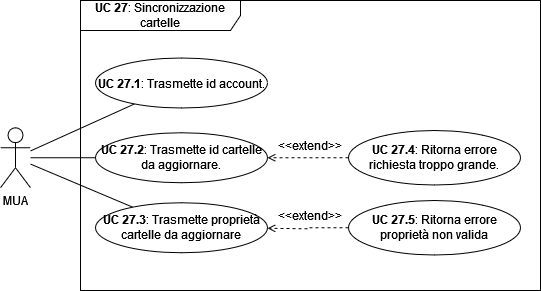
\includegraphics[width=0.85\textwidth]{sections/uc_imgs/UC27.png}
        \centering
        \caption{Sottocasi d'Uso di UC 27}
    \end{figure}

    \subsubsection{UC 27.1 - Trasmette id account} \label{sec:UC27.1}
    \begin{itemize}
        \item \textbf{Attore principale}: MUA;
        \item \textbf{Descrizione}: il MUA invia al sistema l'id dell'account associato all'utente;
        \item \textbf{Precondizioni}: il MUA sta usando la funzionalità di sincronizzazione cartelle;
        \item \textbf{Postcondizioni}: il sistema conosce l'id dell'account;
        \item \textbf{Scenario principale}:
            \begin{enumerate}
                \item il MUA trasmette l'id dell'account associato all'utente al sistema.
            \end{enumerate}
        \item \textbf{Inclusioni}: nessuna;
        \item \textbf{Generalizzazioni}: nessuna;
        \item \textbf{Estensioni}: nessuna.
    \end{itemize}

    \subsubsection{UC 27.2 - Trasmette id cartelle da aggiornare} \label{sec:UC27.2}
    \begin{itemize}
        \item \textbf{Attore principale}: MUA;
        \item \textbf{Descrizione}: il MUA invia al sistema gli id delle cartelle da aggiornare;
        \item \textbf{Precondizioni}: il MUA sta usando la funzionalità di sincronizzazione delle cartelle;
        \item \textbf{Postcondizioni}: il sistema conosce gli id delle cartelle da aggiornare;
        \item \textbf{Scenario principale}:
            \begin{enumerate}
                \item il MUA trasmette gli id delle cartelle da aggiornare.
            \end{enumerate}
        \item \textbf{Inclusioni}: nessuna;
        \item \textbf{Generalizzazioni}: nessuna;
        \item \textbf{Estensioni}:
            \begin{enumerate}[label=\alph*.]
                \item la quantità di cartelle da aggiornare supera la quantità massima di richieste al server:
                \begin{enumerate}[label=\arabic*.]
                    \item il sistema ritorna un errore al MUA di richiesta troppo grande (\hyperref[sec:UC27.4]{UC 27.4}).
                \end{enumerate}
            \end{enumerate}
    \end{itemize}


    \subsubsection{UC 27.3 - Trasmette proprietà cartelle da aggiornare} \label{sec:UC27.3}
    \begin{itemize}
        \item \textbf{Attore principale}: MUA;
        \item \textbf{Descrizione}: il MUA invia al sistema le proprietà delle cartelle da aggiornare;
        \item \textbf{Precondizioni}: il MUA sta usando la funzionalità di sincronizzazione delle cartelle;
        \item \textbf{Postcondizioni}: il sistema conosce quali sono le proprietà delle cartelle da aggiornare;
        \item \textbf{Scenario principale}:
            \begin{enumerate}
                \item il MUA trasmette le proprietà delle cartelle da aggiornare.
            \end{enumerate}
        \item \textbf{Inclusioni}: nessuna;
        \item \textbf{Generalizzazioni}: nessuna;
        \item \textbf{Estensioni}:
            \begin{enumerate}[label=\alph*.]
                \item le proprietà delle cartelle da aggiornare non sono valide:
                \begin{enumerate}[label=\arabic*.]
                    \item il sistema ritorna un errore al MUA di proprietà non valida (\hyperref[sec:UC27.5]{UC 27.5}).
                \end{enumerate}
            \end{enumerate}
    \end{itemize}


    \subsubsection{UC 27.4 - Ritorna errore richiesta troppo grande} \label{sec:UC27.4}
    \begin{itemize}
        \item \textbf{Attore principale}: MUA;
        \item \textbf{Descrizione}: il MUA riceve l'errore che la quantità delle cartelle da aggiornare supera la quantità massima di richieste al server;
        \item \textbf{Precondizioni}: il MUA ha inviato gli id delle cartelle da aggiornare;
        \item \textbf{Postcondizioni}: il sistema non invia gli aggiornamenti e il MUA viene notificato che il numero delle cartelle da aggiornare è eccessivo;
        \item \textbf{Scenario principale}:
            \begin{enumerate}
                \item il sistema verifica la quantità di richieste;
                \item il sistema rileva che il numero di richieste supera la soglia massima consentita;
                \item il sistema non invia gli aggiornamenti e notifica il MUA dell'eccesso di richieste.
            \end{enumerate}
        \item \textbf{Inclusioni}: nessuna;
        \item \textbf{Generalizzazioni}: nessuna;
        \item \textbf{Estensioni}: nessuna.
    \end{itemize}

    \subsubsection{UC 27.5 - Ritorna errore proprietà non valida} \label{sec:UC27.5}
    \begin{itemize}
        \item \textbf{Attore principale}: MUA;
        \item \textbf{Descrizione}: il MUA riceve l'errore che la proprietà delle cartelle da aggiornare non è valida;
        \item \textbf{Precondizioni}: il MUA ha inviato la proprietà delle cartelle da aggiornare;
        \item \textbf{Postcondizioni}: il sistema non invia gli aggiornamenti e il MUA viene notificato che la proprietà delle cartelle da aggiornare non è valida;
        \item \textbf{Scenario principale}:
            \begin{enumerate}
                \item il sistema verifica la validità della proprietà trasmessa e trova un errore;
                \item il sistema non invia gli aggiornamenti e notifica il MUA dell'errore.
            \end{enumerate}
        \item \textbf{Inclusioni}: nessuna;
        \item \textbf{Generalizzazioni}: nessuna;
        \item \textbf{Estensioni}: nessuna.
    \end{itemize}